The major goal of this report is to be able to develop a real-world application. In order to do this, all real-world implications need to be taken into consideration. Scenario's were developed to develop a charging protocol that accounts for all possible states. For these scenarios a user wearing a tranceiver wristband is considered. Other viewpoints for a scenario can be the user wearing a receiving wristband or the transmitting bar. However, these viewpoints are considerably easier to address and will implements parts of the protocol designed for a tranceiving system.

There are certain states in which the system can reside depending on its own battery state, the battery state of neighbour nodes and the availability of a charging bar. These states and their transmissions are displayer in figure \ref{fig:states}. It can either be sufficiently full defined as $V_{full}$, starving defined as $V_{starve}$ or dead which is defined by $V_{dead}$. These parameters are further specified in section \ref{sec:proposed}.

\begin{figure}[h!]
\centering
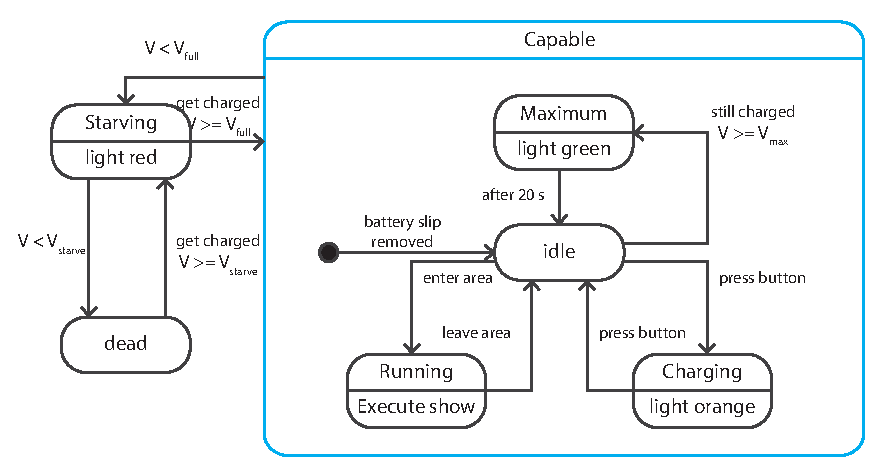
\includegraphics[width=0.8\textwidth]{statediagram.pdf}
\caption{State diagram of a transceiving wireless power transfer system}
\label{fig:states}
\end{figure}

A charging protocol has to be designed to account for these combinations. We considered three possibilities: an infinite network like design, a hop-to-hop spread of energy or an interactive behavior to selectively share energy. To stimulate interaction through this application we choose to apply a scenario where a user can choose to act upon energy requests and share with friends, or strangers.

% add reason why we choose this protocol

To handle these protocols, an IC has to be added. This way whenever the battery reached $V_{starve}$ it will send out a request for energy visually by litting a red LED embedded in the wristband. Neighbouring nodes can then choose to react on this or save their own energy. Whenever the battery dies, the user either has to verbally ask for energy of visit an energy bar.

% make a scenario

